\subsection{Towards robust boosted jet tagging}
When we first studied W-tagging at 13 \TeV in context with the analysis of the 2015 dataset, Section~\ref{sec:searchI:wtagging}, two interesting correlations were observed:

\bigskip
1) A strong dependence of the AK8 CHS softdrop ($\beta = 0$) jet mass on jet \PT and

2) a strong dependence of the AK8 CHS $\tau_{21}$ cut efficiency on pileup.
\bigskip

The reason we studied the softdrop algorithm as an alternative to pruning in 2015 was, besides the possibility it would result in a higher signal efficiency, that we knew it had certain favorable qualities compared to other groomers: Softdrop removes all sensitivity to the soft divergences of QCD, by removing all soft emission, more specifically the non-global logarithmic terms (NGLs) in the jet mass~\cite{Dasgupta:2013ihk}. These arise from constellations where, for instance, a soft gluon is radiated into the jet cone, as illustrated in Figure~\ref{fig:searchII:ngls}. 

\begin{figure}[h!]
\centering
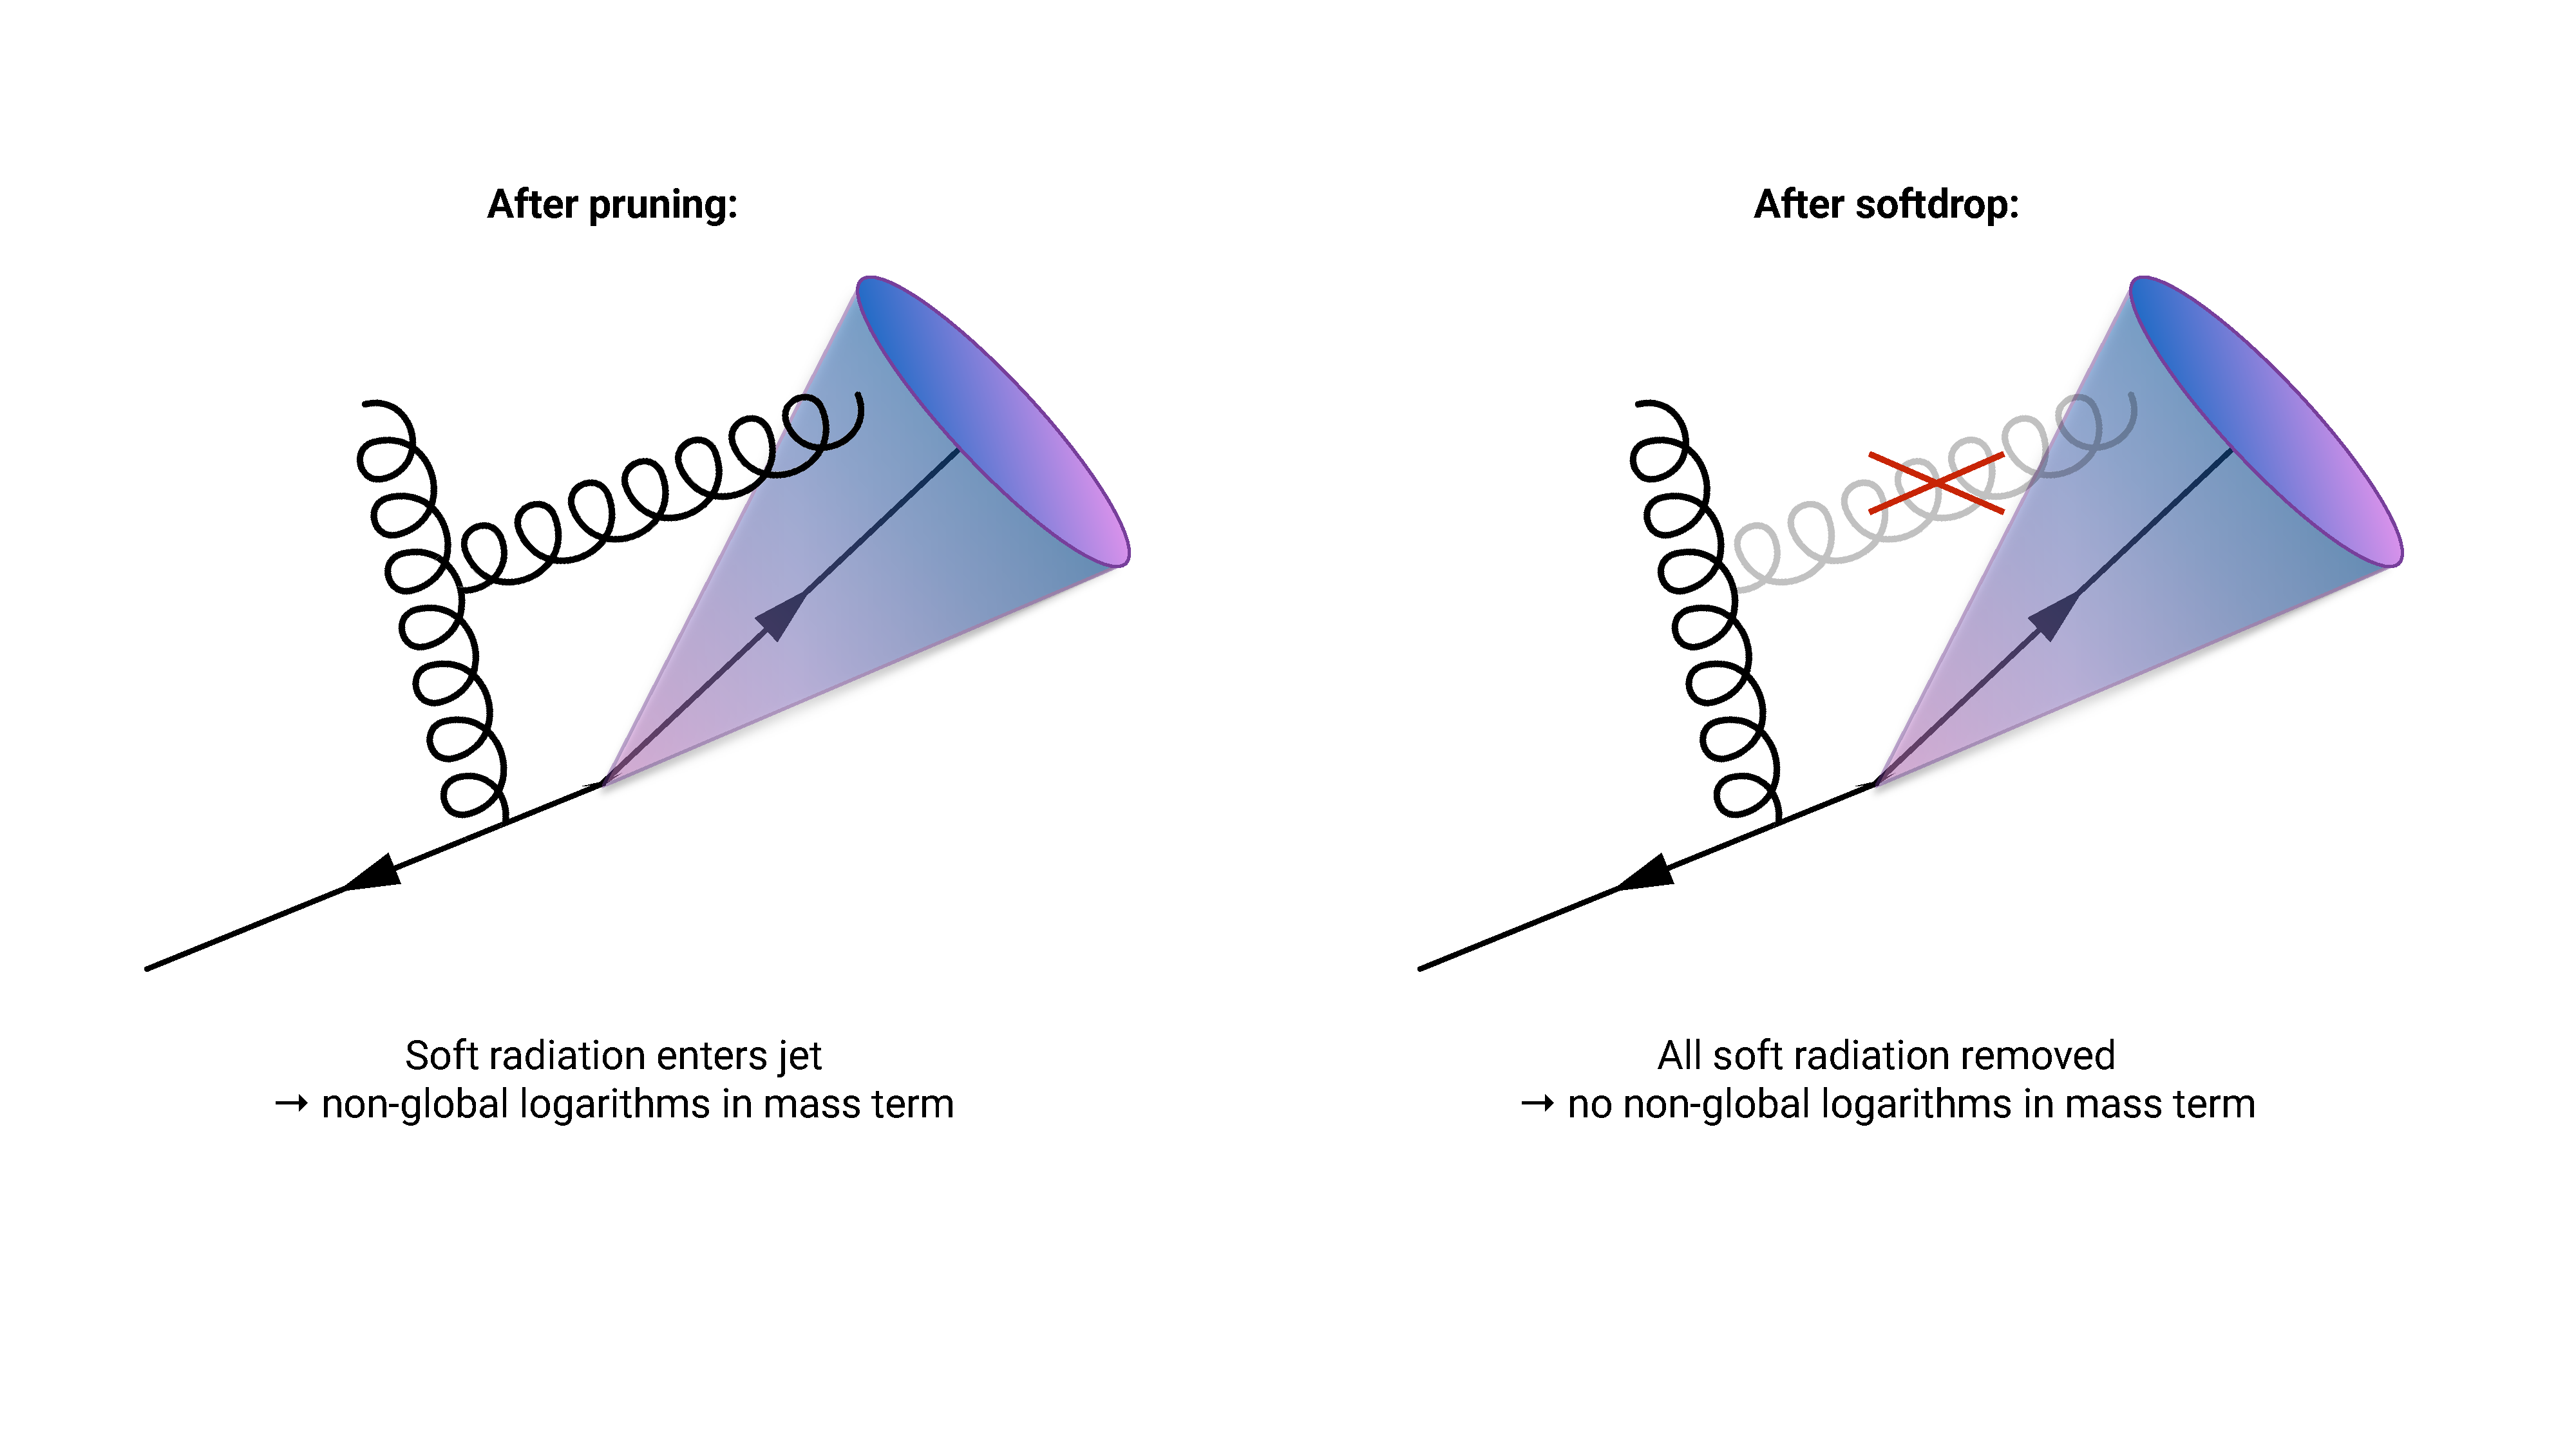
\includegraphics[width=0.79\textwidth]{figures/analysis/search2/misc/ngls.pdf}
\caption{The pruning algorithm does not remove all soft emission and therefore has non-global logarithmic terms in the jet mass. Softdrop ($\beta = 0$) completely removes soft emissions and is therefore free of non-global logarithms.}
\label{fig:searchII:ngls}
\end{figure}

The consequence of this is that you can calculate the softdrop jet mass to way higher precision than what is possible for other grooming algorithms or for the plain jet mass (NGLs are the main reason a full resummation of the plain jet mass beyond NLL (considering e.g multiple-emission effects) accuracy does not exist). Despite this not being a precision measurement analysis, we had theoretically well-motivated reasons for wanting the baseline CMS V-tagger to be softdrop-based.\newline
However, despite being less sensitive to soft radiation for QCD jets, signal jets groomed with softdrop were found to be far more sensitive to the underlying event than pruned jets~\cite{Dasgupta:2015yua}. Figure~\ref{fig:searchII:ue} shows the signal efficiency for pruning (left) and softdrop (right) as a function of jet transverse momenta when including FSR only, FSR+ISR, hadronization and hadronization + underlying event.


\begin{figure}[h!]
\centering
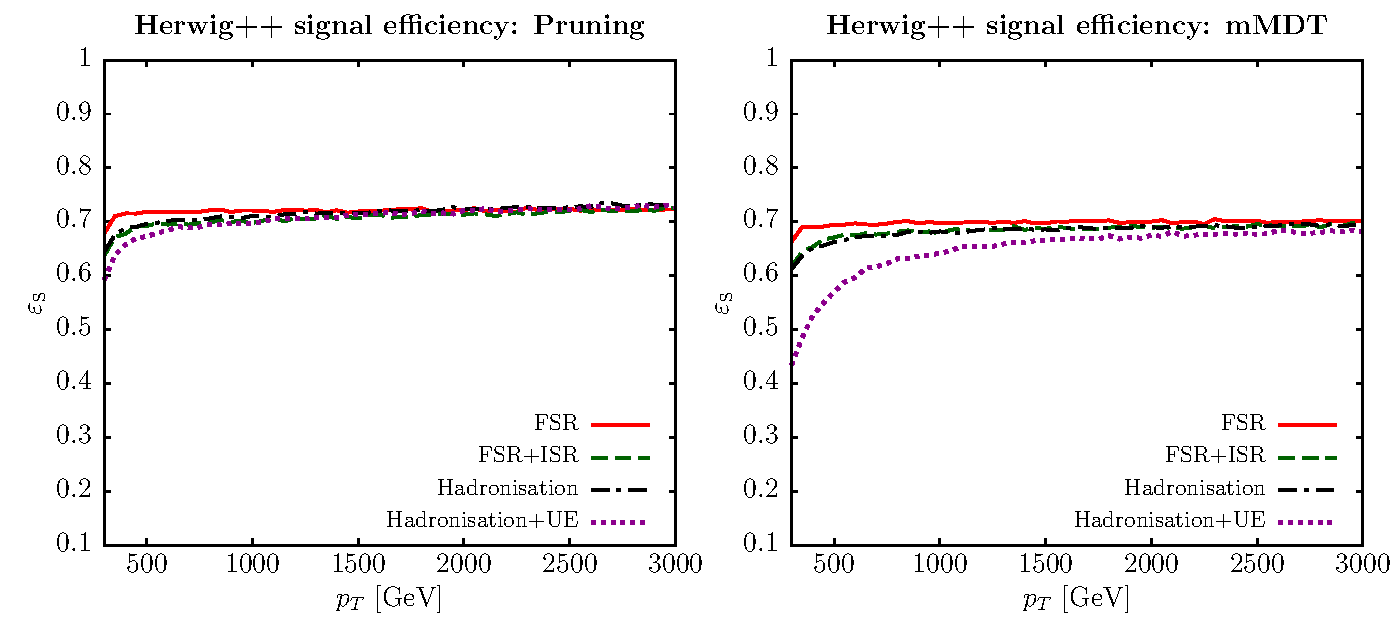
\includegraphics[width=0.99\textwidth]{figures/analysis/search2/misc/pruningvssd_ue.pdf}
\caption{The signal efficiency for pruning (left) and softdrop (right) as a function of jet \PT when adding FSR, ISR, hadronization and UE. THe UE has a severe impact on the softdrop efficiency for signal jets~\cite{Dasgupta:2015yua}. }
\label{fig:searchII:ue}
\end{figure}

On parton level, as well as after hadronization, the two algorithms perform very similar as a function of \PT. However, once UE contamination is added, the softdrop tagging efficiency is severely affected. This can be explained by the larger effective radius considered by the softdrop algorithm ( $\propto \mV/\PT \sqrt{z_{cut}(1-z_{cut})}$ ) in comparison to pruning ( $\propto \mV/\PT$ ). This observation corresponds very well with the shift in jet mass we observed for softdrop as a function of \PT in Section~\ref{sec:searchI:wtagging}: As the jet \PT decreases the softdrop effective radius increases and the jet mass mean shifts to higher values, due to absorbing more background radiation. If softdrop would be our new default tagger, a better rejection of pileup and UE contamination would be needed.
\bigskip
In parallel to the ongoing theoretical work on groomers, a novel pileup removal algorithm had been proposed: Pileup per particle identification (PUPPI)~\cite{Bertolini2014}. Described in detail in Section~\ref{subsub:objreco:puppi}, PUPPI considers not only charged pileup but rather reweights each particle in the jet with its probability of arising from pileup. PUPPI had proven it self far superior to the current CHS algorithm in terms of jet mass resolution for large radius jets, and therefore seemed like the obvious choice to address both issues listed above: The sensitivity of softdrop regarding UE contamination and the strong pileup dependence of $\tau_{21}$.


 

\subsection{Analysis strategy}
\subsection{Developing a new W-tagger}
\label{sec:searchII:puppisoftdrop}